\chapter{System Modeling}
To simulate a steam drum and boiler, a model must be created. A highly praised model used in many other papers is the \r{A}str\"{o}m-Bell non-linear drum-boiler model.\cite{Astrom} This model can be expanded upon as it uses an approximation of steam properties. Expanding the \r{A}str\"{o}m-Bell second order model to a more accurately fit model increases both the accuracy and the computational complexity. The \r{A}str\"{o}m-Bell model can then extended using Iacob and Andreescu's methods \cite{Iacob} to create a reduced order model. Further reductions can be made with a specific set of assumptions and conditions. It can be assumed that several inputs will remain near constant. Also, first order differential equations will be used to approximate the physical dynamics of valves. 

\section{Steam Property Modeling}

    The simulation of a drum boiler requires an understanding of the thermodynamic properties of saturated steam. Saturation temperature, density (specific volume), and enthalpy are all functions of pressure. The \r{A}str\"{o}m-Bell model uses quadratic functions to model these properties. A quadratic function was used because the derivatives of these functions will be used in future calculations, and linear or constant derivatives are produced from quadratic models. Table \ref{table:Steam_ModelingA} shows the exact equations used in the \r{A}str\"{o}m-Bell model. 
    Figure \ref{fig:Curve_Fit_SteamA} shows how these equations compare to the physical properties. Note how at lower pressures there is a high degree of variation. 
    
    \begin{table}[ht]
        \begin{center}
        \begin{scriptsizetabular}{|l|c l|}
            \hline
             &  & Original Model Equation  \\
            \hline
            Saturated Steam Temperature & & $T(p)      = C p^2 + B p + A$ \\ 
            Saturated Vapor Enthalpy    & & $h_s(p)    = C p^2 + B p + A$ \\ 
            Saturated Vapor Density     & & $\rho_s(p) = C p^2 + B p + A$ \\ 
            Saturated Liquid Enthalpy   & & $h_w(p)    = C p^2 + B p + A$ \\ 
            Saturated Liquid Density    & & $\rho_w(p) = C p^2 + B p + A$ \\ 
            \hline
        \end{scriptsizetabular}
        \caption{Original Steam Table Models}
        \label{table:Steam_ModelingA}
        \end{center}
    \end{table}
    
    \begin{figure}[ht]
        \begin{center}
        \resizebox{\ScaleMLFigSteam \textwidth}{!}{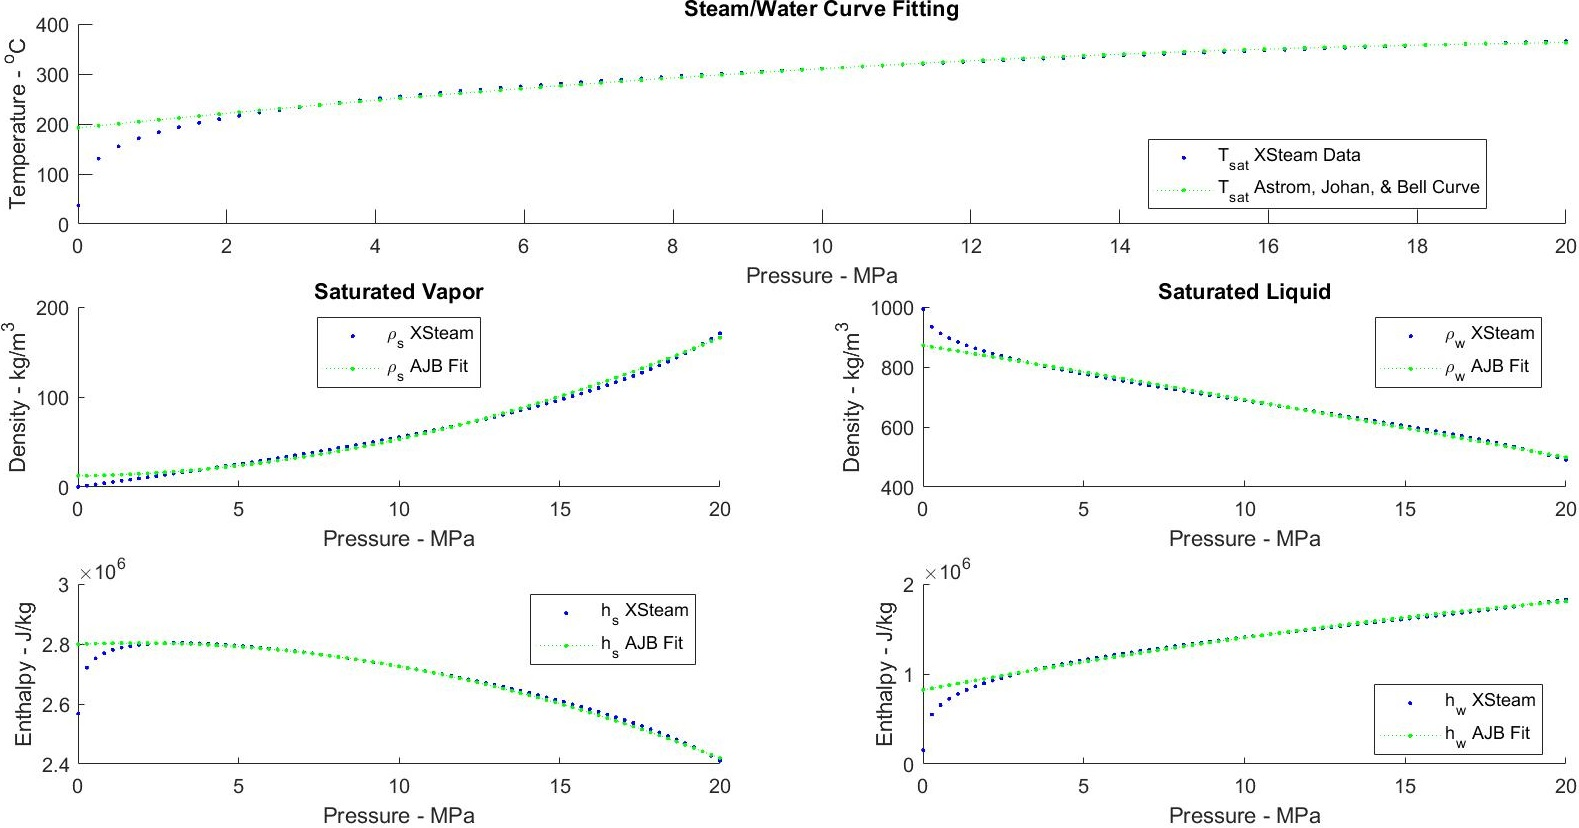
\includegraphics{Modeling/Steam/Steam_Table_Curve_Fits_Original}}
        \caption{Curve Fitting Steam}
        \label{fig:Curve_Fit_SteamA}
        \end{center}
    \end{figure}
    
    A more elaborate model can be used, and a curve fitting process can be applied to the tables of physical properties. The advantage of using a more elaborate model is that the operating parameters can be further expanded outside of the range of where the quadratic model breaks down. The various model types are defined in Table \ref{table:Steam_ModelingB}. Exponential and cubic equations were used for a more accurate fit. Figure \ref{fig:Curve_Fit_SteamB} shows the steam properties table, the quadratic model, and an expanded model. 
    
    \begin{figure}[ht]
        \begin{center}
        \resizebox{\ScaleMLFigSteam \textwidth}{!}{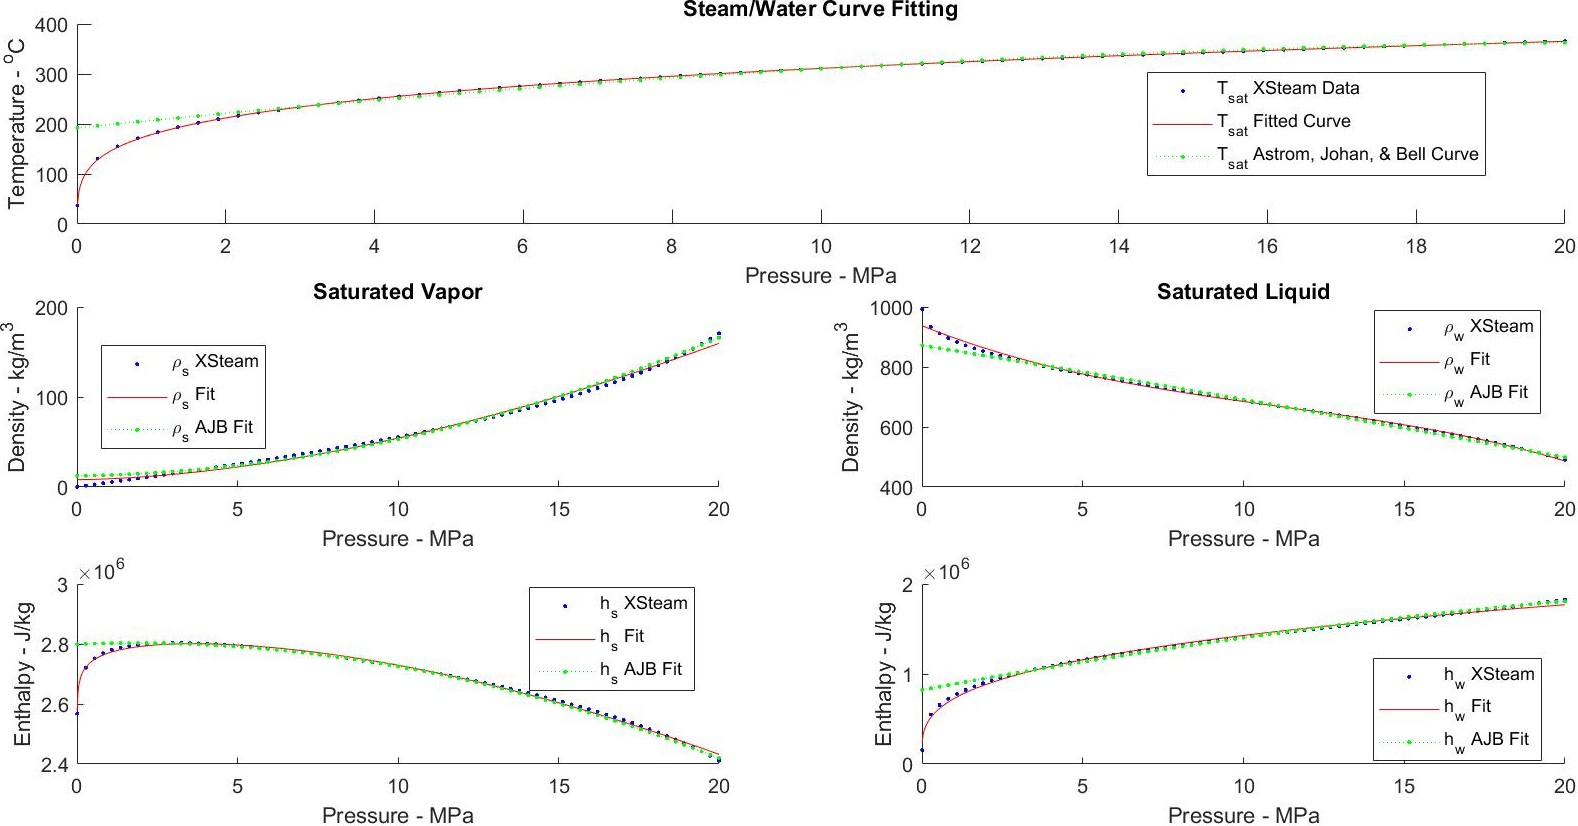
\includegraphics{Modeling/Steam/Steam_Table_Curve_Fits}}
        \caption{Curve Fitting Steam}
        \label{fig:Curve_Fit_SteamB}
        \end{center}
    \end{figure}
    
    \begin{table}[ht]
        \begin{center}
        \begin{scriptsizetabular}{|l| c l l|}
            \hline
              & & Original Model Equation & Expanded Model Equation \\
            \hline
            Saturated Steam Temperature & & $T(p)      = C p^2 + B p + A$ & $T(p)      = Bp^C +A$\\ 
            Saturated Vapor Enthalpy    & & $h_s(p)    = C p^2 + B p + A$ & $h_s(p)    = Dp^E + Bp^C+A$\\ 
            Saturated Vapor Density     & & $\rho_s(p) = C p^2 + B p + A$ & $\rho_s(p) = Bp^C +A$\\ 
            Saturated Liquid Enthalpy   & & $h_w(p)    = C p^2 + B p + A$ & $h_w(p)    = Bp^C +A$\\ 
            Saturated Liquid Density    & & $\rho_w(p) = C p^2 + B p + A$ & $\rho_w(p) = Dp^3 + C p^2 + B p + A$ \\
            \hline
        \end{scriptsizetabular}
        \caption{Expanded Steam Table Models}
        \label{table:Steam_ModelingB}
        \end{center}
    \end{table}    
    
    It is clear from Figure \ref{fig:Curve_Fit_SteamB} that the more complex exponential models are a better fit than the quadratic modeling, as the model does not break down in the lower pressure ranges. While the original quadratic model makes the math much simpler when performing the partial derivatives the use of computational tools (MatLab's Symbolic Toolbox) makes this a rewarding design trade off when compared to the expanded pressure ranges that the new model can operate at and the trivial nature of calculating these partial derivatives. 
    
\section{\r{A}str\"{o}m and Bell Model}

    \r{A}str\"{o}m and Bell's goal in creating a model was to find a moderately complex nonlinear model that captured the key properties of shrink and swell for drum boiler level. A first order model can be used if drum level is considered well controlled. The first order model ignores the drum level and therefore cannot be used for the purposes of this paper. \cite{Astrom}
    
    \subsection{Global Mass and Energy Balance}
    
        The global Mass balance is: 
        $$\frac{\mathrm{d} }{\mathrm{d} t}\left [ \rho_s V_{st} + \rho_w V_{wt}\right ] = q_f - q_s$$\cite{Astrom}
        This can be placed into words as the sum of the change in the mass of the steam and water in the system (calculated as $m = \rho V$) must be equal to the sum of the mass flow rate of the steam flow out of the system and feed-water flow into the system. This is the principle of the conservation of mass. 
        
        The global mass balance can be placed into matrix form with some manipulations to become Eq. \eqref{eq:Mass_Balance} noting that $\rho$ is a function of $p$. \cite{Astrom}
        \begin{equation}
            \label{eq:Mass_Balance}
            \left [ \begin{matrix} e_{11}& e_{12}\end{matrix} \right ] \frac{\mathrm{d} }{\mathrm{d} t} \left [ \begin{matrix} V_{wt}\\ p\end{matrix} \right ] = q_f  - q_s
        \end{equation}
        In Eq. \ref{eq:Mass_Balance} the coefficients are defined as follows:
        \begin{equation*}
                e_{11}      = \rho_w - \rho_s
        \end{equation*}
        \begin{equation*}
                e_{12}      = V_{wt} \frac{\partial \rho_w }{\partial p} - V_{st} \frac{\partial \rho_s }{\partial p}
        \end{equation*}
        
        The global energy balance is 
        $$\frac{\mathrm{d} }{\mathrm{d} t}\left [ \rho_s h_s V_{st} + \rho_w h_w V_{wt} - pV_t + m_tC_pt_m\right ] = Q + q_f h_f - q_s h_s $$\cite{Astrom}
        This can be placed into words as the change of internal energy in both steam and water and the change of energy due to the change in volume and the temperature of the metal must equal the sum of the heat transfer in, the energy the steam brings, and the energy the feed-water brings. 
        
        The global energy balance can be simplified to become:\cite{Astrom}
        \begin{equation}
            \label{eq:Energy_Balance}
            \left [ \begin{matrix} e_{21}& e_{22}\end{matrix} \right ] \frac{\mathrm{d} }{\mathrm{d} t} \left [ \begin{matrix} V_{wt}\\ p\end{matrix} \right ] = Q + q_f h_f  - q_s h_s 
        \end{equation}
        In Eq \ref{eq:Energy_Balance} the coefficients are defined as follows:
        \begin{equation*}
            e_{21} = \rho_w h_w - \rho_s h_s 
        \end{equation*}
        \begin{equation*}
            e_{22} = V_{wt} \left ( h_w  \frac{\partial \rho_w }{\partial p} + \rho_w \frac{\partial h_w }{\partial p}\right ) + V_{st} \left ( h_s  \frac{\partial \rho_s }{\partial p} + \rho_s \frac{\partial h_s }{\partial p}\right ) - V_{t} + m_t C_p \frac{\partial t_s }{\partial p}
        \end{equation*}
        
        %It should be noted that for Mass and Energy balance alone, Equations \eqref{eq:Mass_Balance}-\eqref{eq:Energy_Balance} are enough to create a simple model, however this model is not sufficient to capture the drum level dynamics. 
        %\begin{equation}
        %    \label{eq:Mass_Energy_BalanceA}
        %    \left [ \begin{matrix} e_{11}& e_{12} \\ e_{21}& e_{22}\end{matrix} \right ] \frac{\mathrm{d} }{\mathrm{d} t} \left [ \begin{matrix} V_{wt}\\ p\end{matrix} \right ] =  \left [ \begin{matrix} q_f  - q_s \\ Q + q_f h_f  - q_s h_s \end{matrix} \right ]
        %\end{equation}        
        
        %For future calculations, the Mass and Energy Balance equations \eqref{eq:Mass_Energy_BalanceA} will be expanded trivially into Equation \eqref{eq:Mass_Energy_Balance}. Please note that $\alpha_r$ and $V_{sd}$ will be defined as states and used later. 
        %\begin{equation}
        %    \label{eq:Mass_Energy_Balance}
        %    \left [ \begin{matrix} e_{11}& e_{12} & 0& 0\\ e_{21}& e_{22}& 0& 0\end{matrix} \right ] %\frac{\mathrm{d} }{\mathrm{d} t} \left [ \begin{matrix} V_{wt}\\ p\\ \alpha_r\\ V_{sd}\end{matrix} %\right ] =  \left [ \begin{matrix} q_f  - q_s \\ Q + q_f h_f  - q_s h_s \end{matrix} \right ]
        %\end{equation}           

    \subsection{Distribution of Steam in Risers and Drum}
    
    
        The energy balance for the riser section:
        $$\frac{\mathrm{d} }{\mathrm{d} t}\left [ \rho_s h_s \overline{\alpha}_v V_{r} + \rho_w h_w\left ( 1 - \overline{\alpha}_v \right ) V_{r} - pV_r + m_r C_p t_s\right ] = Q + q_{dc} h_w - \left ( \alpha_r h_c + h_w \right )q_{r} $$\cite{Astrom}
        This can be placed into words as the change of internal energy in both steam and water in the risers and the change of energy due to the change in volume and the temperature of the metal of the risers  must equal the sum of the heat transfer in, the energy the risers looses, and the energy the water in the down comers brings. $\overline{\alpha}_v$ is the average steam volume ratio.
        
        The riser section energy balance can be simplified to become:\cite{Astrom}
        \begin{equation}
            \label{eq:Riser_Energy_Balance}
            \left [ \begin{matrix}  e_{32}& e_{33}\end{matrix} \right ] \frac{\mathrm{d} }{\mathrm{d} t} \left [ \begin{matrix}  p\\ \alpha_r\end{matrix} \right ] = Q + \alpha_r h_c q_{dc} 
        \end{equation}
        
        \clearpage
    
        In Eq \ref{eq:Riser_Energy_Balance} the coefficients are defined as follows:
        
        
        
        \begin{equation*}
            \aligned
                e_{32}  =& \left ( \rho_w \frac{\partial h_w }{\partial p} + \rho_s \frac{\partial h_s }{\partial p}\right )\left ( 1-\overline{\alpha}_v \right )V_r + \left ( \left ( 1- \alpha_r \right ) h_c \frac{\partial \rho_s }{\partial p} + \rho_s \frac{\partial h_s }{\partial p} \right ) \overline{\alpha}_v V_r \\
                         &+  \left (  \rho_s + \left ( \rho_w - \rho_s \right )\alpha_r \right ) h_c V_r \frac{\partial \overline{\alpha}_v }{\partial p}  - V_r+m_r C_p \frac{\partial t_s }{\partial p}
                \endaligned
        \end{equation*}
        

        \begin{equation*}
            e_{33}  = \left ( \left ( 1-\alpha_r \right )\rho_s + \alpha_r \rho_w \right )h_c V_r \frac{\partial \overline{\alpha}_v }{\partial \alpha_r} 
        \end{equation*}
        
        The mass balance for the riser section is:
        $$\frac{\mathrm{d} }{\mathrm{d} t}\left [ \rho_s \overline{\alpha}_v V_{r} + \rho_w \left ( 1 - \overline{\alpha}_v \right )V_{r} \right ] = q_{dc}-q_{r} $$\cite{Astrom}
        This can be placed into words as the change in density and volume of both steam and water in the risers must be equal to the mass flow rate of the sum of the mass flow rates into the down comers and out of the risers.  
        
        The riser section mass balance can be simplified to become:
        \begin{equation}
            \label{eq:Riser_Mass_Balance}
            \left [ \begin{matrix}  e_{42}& e_{43}& e_{44}\end{matrix} \right ] \frac{\mathrm{d} }{\mathrm{d} t} \left [ \begin{matrix} p\\ \alpha_r\\ V_{sd}\end{matrix} \right ] = \frac{\rho_s}{T_d}  \left ( V_{sd}^0  - V_{sd}\right ) + \frac{h_f - h_w}{h_c}q_f
        \end{equation}
        
        In Eq \ref{eq:Riser_Mass_Balance} the coefficients are defined as follows:\cite{Astrom}

        
        \begin{equation*}
            \aligned
                e_{42} = & V_{sd}\frac{\partial \rho_s }{\partial p} + \frac{1}{h_c}\left ( \rho_s V_{sd} \frac{\partial h_s }{\partial p} + \rho_w V_{wd} \frac{\partial h_w }{\partial p} - V_{sd} - V_{wd} + m_d C_p \frac{\partial t_s }{\partial p} \right ) \\
                &+ \alpha_r\left ( 1+\beta \right )V_r \left ( \overline{\alpha}_v \frac{\partial \rho_s }{\partial p} + \left ( 1-\overline{\alpha}_v \right )\frac{\partial \rho_w }{\partial p} + \left ( \rho_s - \rho_w \right ) \frac{\partial \overline{\alpha}_v }{\partial p} \right )
            \endaligned
        \end{equation*}
        

        \begin{equation*}
            e_{43} = \alpha_r\left ( 1+\beta \right )\left ( \rho_s - \rho_w \right )V_r\frac{\partial \overline{\alpha}_v }{\partial p}
        \end{equation*}
        \begin{equation*}    
            e_{44} = \rho_s
        \end{equation*}

\section{Simulation of \r{A}str\"{o}m and Bell Model}
    
    Equations \ref{eq:Mass_Balance}, \ref{eq:Energy_Balance}, \ref{eq:Riser_Energy_Balance}, and  \ref{eq:Riser_Mass_Balance} can be combined to give the following equation :

    $$\left [ \begin{matrix}e_{11}& e_{12}& 0& 0 \\ e_{21}& e_{22}& 0& 0 \\ 0 & e_{32}& e_{33}& 0 \\ 0 & e_{42}& e_{43}& e_{44}\end{matrix} \right ] \frac{\mathrm{d} }{\mathrm{d} t} \left [ \begin{matrix} V_{wt}\\ p\\ \alpha_r\\ V_{sd}\end{matrix} \right ] = \left [ \begin{matrix} q_f  - q_s \\ Q + q_f h_f  - q_s h_s\\ Q + \alpha_r h_c q_{dc} \\ \frac{\rho_s}{T_d}  \left ( V_{sd}^0  - V_{sd}\right ) + \frac{h_f - h_w}{h_c}q_f \end{matrix} \right ]$$

    \begin{equation}
        \label{eq:Model_1}
        \frac{\mathrm{d} }{\mathrm{d} t} \left [ \begin{matrix} V_{wt}\\ p\\ \alpha_r\\ V_{sd}\end{matrix} \right ] =
        \left [ \begin{matrix}e_{11}& e_{12}& 0& 0 \\ e_{21}& e_{22}& 0& 0 \\ 0 & e_{32}& e_{33}& 0 \\ 0 & e_{42}& e_{43}& e_{44}\end{matrix} \right ] ^{-1} \left [ \begin{matrix} q_f  - q_s \\ Q + q_f h_f  - q_s h_s\\ Q + \alpha_r h_c q_{dc} \\ \frac{\rho_s}{T_d}  \left ( V_{sd}^0  - V_{sd}\right ) + \frac{h_f - h_w}{h_c}q_f \end{matrix} \right ]
    \end{equation}
    
    This can be considered a nonlinear state space model, which takes the form of 
    $$\dot{x}(t) = F\left ( x(t),u(t) \right )$$
    Where Eq \ref{eq:Model_1} uses the following as states:
    $$ \begin{matrix} V_{wt} & p& \alpha_r& V_{sd}\end{matrix} $$
    and where Eq \ref{eq:Model_1} uses the following as Inputs:
    $$ \begin{matrix} q_f & q_s & Q & t_f\end{matrix} $$
    
    For purposes of boiler control, the two requested outputs to be predicted are drum level and drum pressure, both of which may be measured directly using simple sensors. The Nonlinear State Space output equation takes the following form: 
    $$y(t) = G\left ( x(t),u(t) \right )$$
    where the control outputs can be calculated as seen in Equation \ref{eq:Model_1_output}. Where $V_{wd}$ is a known function of the states and inputs and $A_d$ is a constant. 
    \begin{equation}
        \label{eq:Model_1_output}
        y(t) = \left [ \begin{matrix} l\\ p \end{matrix} \right ] = \left [ \begin{matrix} \frac{V_{sd} + V_{wd}}{A_d}\\ p \end{matrix} \right ]= \left [ \begin{matrix} \frac{x_4 + V_{wd}}{A_d}\\ x_2 \end{matrix} \right ]
    \end{equation}
    
    If access to all of the states is possible, it allows for calculations of far more outputs. These include: the level contributions from both steam and water, riser and down comer mass flow rate, total water volume, volume of steam in the drum, condensation flow rate, and the average steam volume ratio. These values are of interest, as they give insight into the boiler dynamics, however they are not required for control. The expanded output equations can be seen below:
    $$y_{expanded}(t) = \left [ \begin{matrix} l\\ p \\ \vdots \end{matrix} \right ] $$
    
    \subsection{Equilibrium Values}
    
        To find the equilibrium point of the system, Eq \ref{eq:Model_1} is set to 0. Then from an operating point, the equations are solved.
        
        The operating point chosen are:
        $$ \begin{matrix} V_{wt0}     & = &   57.1 & & & Q_{0}  & = & 86.78\\ 
                          p_0         & = &    8.5 & & & q_{f0} & = & 50.8\\ 
                          \alpha_{r0} & = & 0.0524 & & & t_{f0} & = & 247.66\\ 
                          V_{sd0}     & = &    4.9 & & & q_{s0} & = & 50.8
                          \end{matrix} $$
                  
    \subsection{Comparison of simulation and \r{A}str\"{o}m and Bell's previous work}

        Validation of the reproduced \r{A}str\"{o}m and Bell model was done by simulating step inputs of the model used in Eq. \eqref{eq:Model_1} and comparing the results to the results of the simulated step inputs that \r{A}str\"{o}m and Bell published. 
        
        The following figures were taken from \r{A}str\"{o}m and Bell's paper, section 5. These are used to directly compare the model generated matches the model, as not all parameters were given. 
        
        % Figure 4 Caption: Responses to a step corresponding to 10 MW in fuel flow rate at medium load
        % Figure 5 Caption: Responses to a step change of 10 kg/s in steam flow rate at medium load
        % Figure 6 Caption: Responses to a step corresponding to 10 MW in fuel flow rate at medium (solid) and high (dashed) loads
        % Figure 7 Caption: Responses to a step change of 10 kg/s in steam flow rate at medium (solid) and high (dashed) loads
        % Figure 8 Caption: Responses to a step change of 10 kg/s in feed water flow rate at medium (solid) and high (dashed) loads
        % Figure 9 Caption: Responses to a step change of 10$^O$ C in feed water temperature at medium (solid) and high (dashed) loads
        
        10 MW fuel flow Step Responses: Figures \ref{fig:Fig6A} - \ref{fig:Fig4D}
        
        \begin{figure}[ht]
            \begin{center}
                \resizebox{\ScaleABFigThree \textwidth}{!}{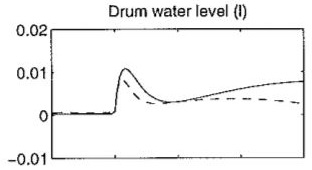
\includegraphics{Modeling/4State/AB_Figures/Figure6/Figure6-AB-1}}
                
                Figure 6 from \r{A}str\"{o}m and Bell's paper, section 5 \cite{Astrom}
                
                \resizebox{\ScaleMLFigThree \textwidth}{!}{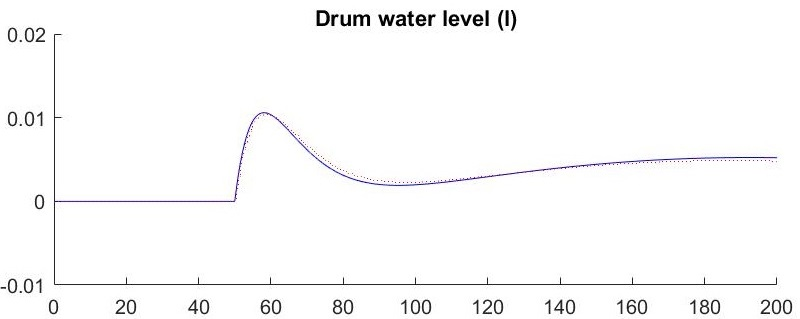
\includegraphics{Modeling/4State/Matlab/Figure12/Figure12-1}}
                
                Simulation Results using Model from Eq \eqref{eq:Model_1}
                
                \caption{Drum Water Level Response to a step corresponding to 10 MW in fuel flow rate}
                \label{fig:Fig6A}
                
            \end{center}
        \end{figure}  % Level
        \begin{figure}[ht]
            \begin{center}
                 \resizebox{\ScaleABFigThree \textwidth}{!}{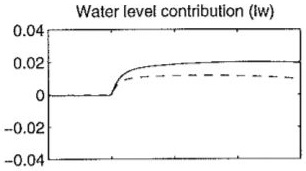
\includegraphics{Modeling/4State/AB_Figures/Figure6/Figure6-AB-3}}
                
                Figure 6 from \r{A}str\"{o}m and Bell's paper, section 5 \cite{Astrom}

                \resizebox{\ScaleMLFigThree \textwidth}{!}{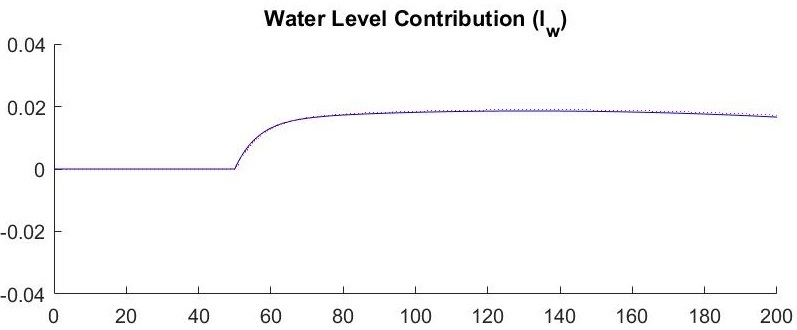
\includegraphics{Modeling/4State/Matlab/Figure12/Figure12-3}}
                
                Simulation Results using Model from Eq \eqref{eq:Model_1}
                
                \caption{Water Level Contribution to a step corresponding to 10 MW in fuel flow rate}
                \label{fig:Fig6B}
            \end{center}
        \end{figure}  % Level Water Contribution
        \begin{figure}[ht]
            \begin{center}
                \resizebox{\ScaleABFigThree \textwidth}{!}{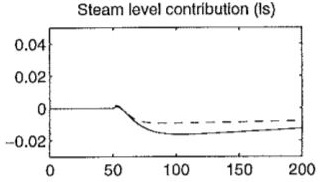
\includegraphics{Modeling/4State/AB_Figures/Figure6/Figure6-AB-5}}
                
                Figure 6 from \r{A}str\"{o}m and Bell's paper, section 5 \cite{Astrom}    
                
                \resizebox{\ScaleMLFigThree \textwidth}{!}{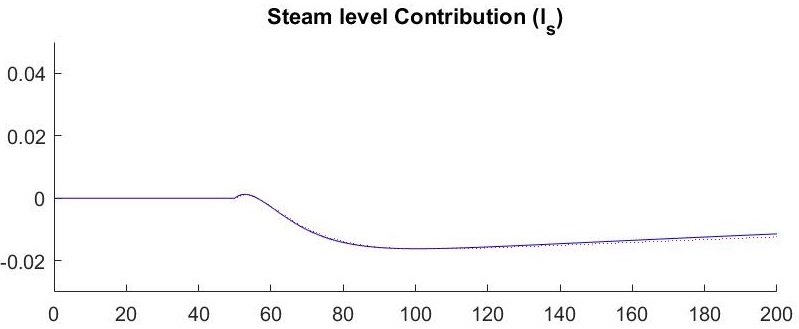
\includegraphics{Modeling/4State/Matlab/Figure12/Figure12-5}}
                
                Simulation Results using Model from Eq \eqref{eq:Model_1}
                
                \caption{Steam Level Contribution to a step corresponding to 10 MW in fuel flow rate}
                \label{fig:Fig6C}
            \end{center}
        \end{figure}  % Level Steam Contribution    
            
        \begin{figure}[ht]
            \begin{center}
                \resizebox{\ScaleABFigThree \textwidth}{!}{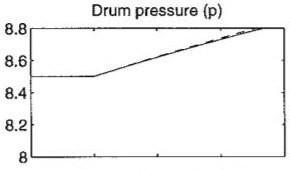
\includegraphics{Modeling/4State/AB_Figures/Figure6/Figure6-AB-2}}
                
                Figure 6 from \r{A}str\"{o}m and Bell's paper, section 5 \cite{Astrom}
                    
                \resizebox{\ScaleMLFigThree \textwidth}{!}{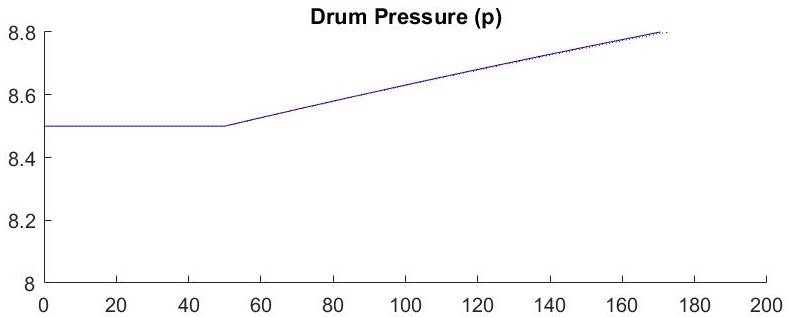
\includegraphics{Modeling/4State/Matlab/Figure12/Figure12-2}}
                
                Simulation Results using Model from Eq \eqref{eq:Model_1}
                
                \caption{Drum Pressure Response to a step corresponding to 10 MW in fuel flow rate}
                \label{fig:Fig6D}                
            \end{center}
        \end{figure}  % Drum Pressure
        \begin{figure}[ht]
            \begin{center}
                \resizebox{\ScaleABFigThree \textwidth}{!}{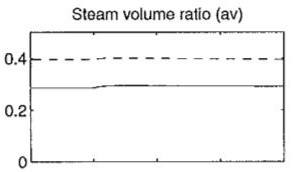
\includegraphics{Modeling/4State/AB_Figures/Figure6/Figure6-AB-4}}
                    
                Figure 6 from \r{A}str\"{o}m and Bell's paper, section 5 \cite{Astrom}
                
                \resizebox{\ScaleMLFigThree \textwidth}{!}{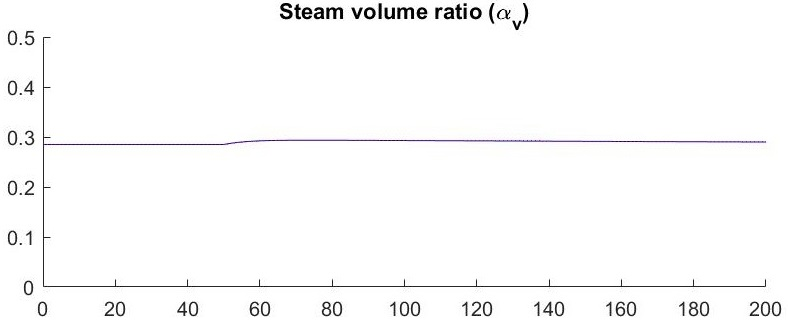
\includegraphics{Modeling/4State/Matlab/Figure12/Figure12-4}}
                
                Simulation Results using Model from Eq \eqref{eq:Model_1}
                
                \caption{Steam Volume Ratio Response to a step corresponding to 10 MW in fuel flow rate}
                \label{fig:Fig6E}
            \end{center}
        \end{figure}  % Steam Volume Ratio 
        \begin{figure}[ht]
            \begin{center}
                \resizebox{\ScaleABFigThree \textwidth}{!}{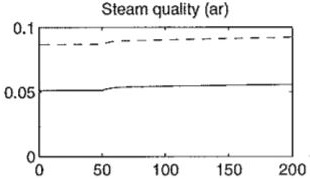
\includegraphics{Modeling/4State/AB_Figures/Figure6/Figure6-AB-6}}
                
                Figure 6 from \r{A}str\"{o}m and Bell's paper, section 5 \cite{Astrom}    
                
                \resizebox{\ScaleMLFigThree \textwidth}{!}{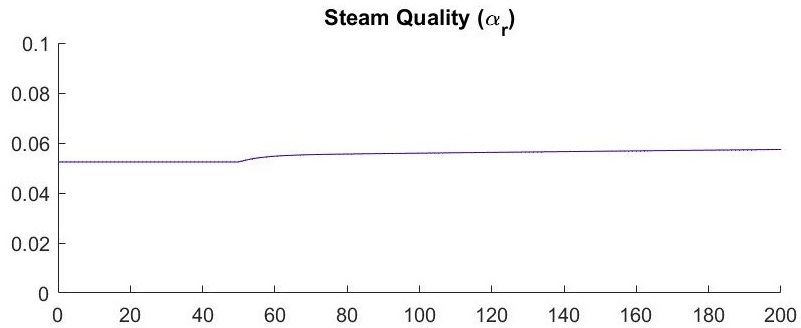
\includegraphics{Modeling/4State/Matlab/Figure12/Figure12-6}}
                
                Simulation Results using Model from Eq \eqref{eq:Model_1}
                
                \caption{Steam Quality Response to a step corresponding to 10 MW in fuel flow rate}
                \label{fig:Fig6F}
            \end{center}
        \end{figure}  % Steam Quality

        \begin{figure}[ht]
            \begin{center}
                \resizebox{\ScaleABFigThree \textwidth}{!}{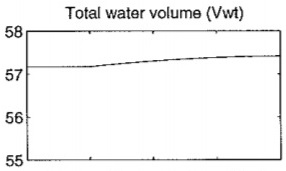
\includegraphics{Modeling/4State/AB_Figures/Figure4/Figure4-AB-2}}
                
                Figure 4 from \r{A}str\"{o}m and Bell's paper, section 5 \cite{Astrom}    
                
                \resizebox{\ScaleMLFigThree \textwidth}{!}{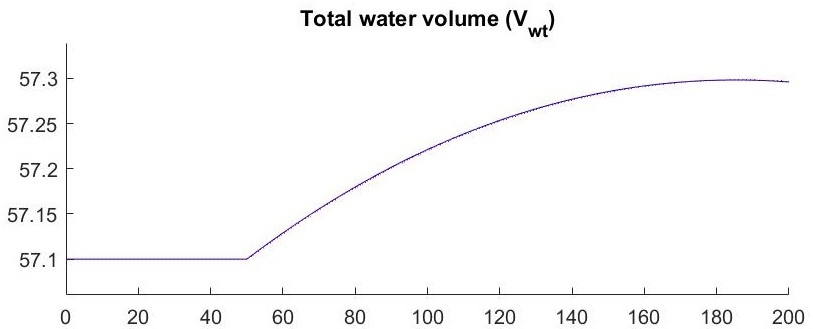
\includegraphics{Modeling/4State/Matlab/Figure11/Figure11-2}}
                
                Simulation Results using Model from Eq \eqref{eq:Model_1}
                
                \caption{Total Water Volume Response to a step corresponding to 10 MW in fuel flow rate}
                \label{fig:Fig4A}
            \end{center}
        \end{figure}
        \begin{figure}[ht]
            \begin{center}
                \resizebox{\ScaleABFigThree \textwidth}{!}{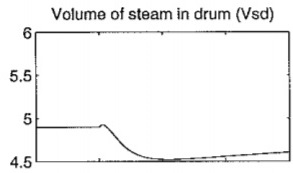
\includegraphics{Modeling/4State/AB_Figures/Figure4/Figure4-AB-4}}
                
                Figure 4 from \r{A}str\"{o}m and Bell's paper, section 5 \cite{Astrom}    
                
                \resizebox{\ScaleMLFigThree \textwidth}{!}{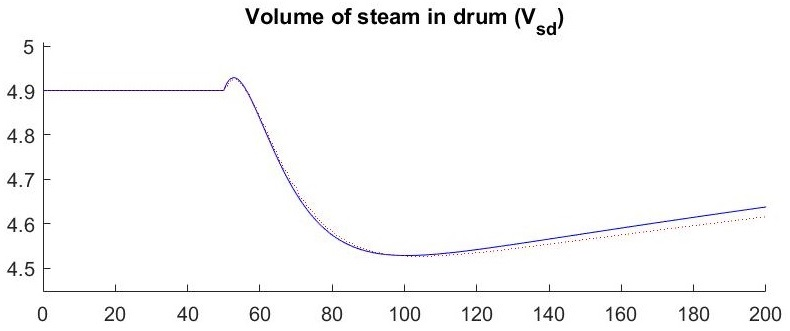
\includegraphics{Modeling/4State/Matlab/Figure11/Figure11-4}}
                
                Simulation Results using Model from Eq \eqref{eq:Model_1}
                
                \caption{Volume of Steam in Drum Response to a step corresponding to 10 MW in fuel flow rate}
                \label{fig:Fig4B}                
            \end{center}
        \end{figure}
        \begin{figure}[ht]
            \begin{center}
                \resizebox{\ScaleABFigThree \textwidth}{!}{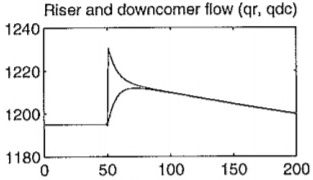
\includegraphics{Modeling/4State/AB_Figures/Figure4/Figure4-AB-5}}
                
                Figure 4 from \r{A}str\"{o}m and Bell's paper, section 5 \cite{Astrom}    
                
                \resizebox{\ScaleMLFigThree \textwidth}{!}{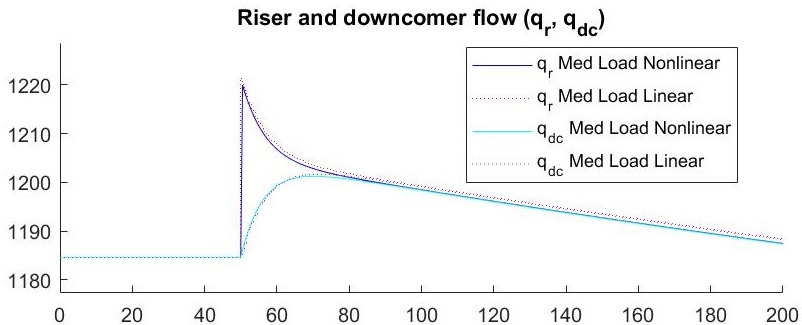
\includegraphics{Modeling/4State/Matlab/Figure11/Figure11-5}}
                
                Simulation Results using Model from Eq \eqref{eq:Model_1}
                
                \caption{Riser and Downcomer Flow Response to a step corresponding to 10 MW in fuel flow rate}
                \label{fig:Fig4C}
            \end{center}
        \end{figure}
        \begin{figure}[ht]
            \begin{center}
                \resizebox{\ScaleABFigThree \textwidth}{!}{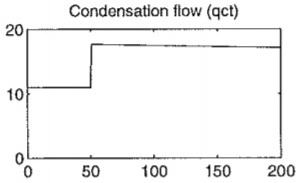
\includegraphics{Modeling/4State/AB_Figures/Figure4/Figure4-AB-6}}
                
                Figure 4 from \r{A}str\"{o}m and Bell's paper, section 5 \cite{Astrom}
                
                \resizebox{\ScaleMLFigThree \textwidth}{!}{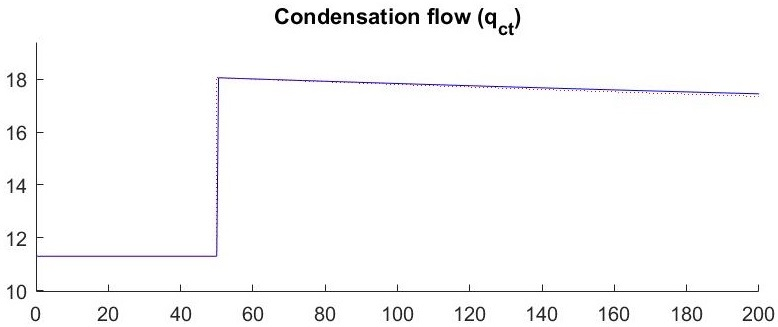
\includegraphics{Modeling/4State/Matlab/Figure11/Figure11-6}}
                
                Simulation Results using Model from Eq \eqref{eq:Model_1}
                
                \caption{Condensation Flow Response to a step corresponding to 10 MW in fuel flow rate}
                \label{fig:Fig4D}
            \end{center}
        \end{figure}            
        
        10 kg/s in steam flow Step Responses: Figures \ref{fig:Fig7A} - \ref{fig:Fig5D}
        \begin{figure}[ht]
            \begin{center}
                \resizebox{\ScaleABFigThree \textwidth}{!}{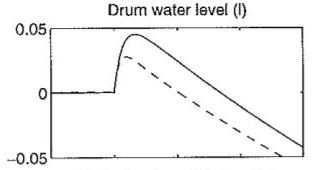
\includegraphics{Modeling/4State/AB_Figures/Figure7/Figure7-AB-1}}
                
                Figure 7 from \r{A}str\"{o}m and Bell's paper, section 5 \cite{Astrom}
                
                \resizebox{\ScaleMLFigThree \textwidth}{!}{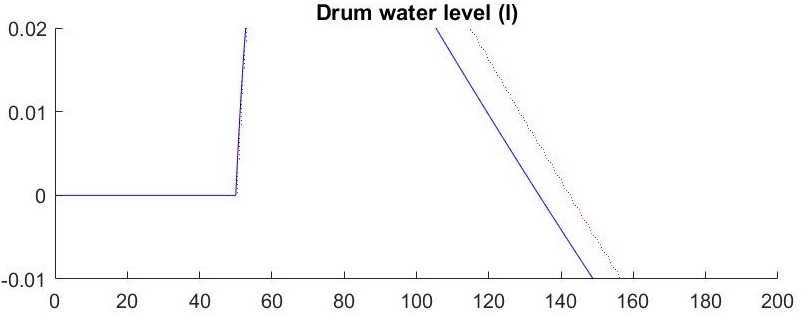
\includegraphics{Modeling/4State/Matlab/Figure22/Figure22-1}}
                
                Simulation Results using Model from Eq \eqref{eq:Model_1}
                
                \caption{Drum Water Level Response to a step change of 10 kg/s in steam flow rate}
                \label{fig:Fig7A}
            \end{center}
        \end{figure}  % Level
        \begin{figure}[ht]
            \begin{center}
                \resizebox{\ScaleABFigThree \textwidth}{!}{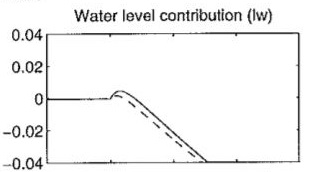
\includegraphics{Modeling/4State/AB_Figures/Figure7/Figure7-AB-3}}
                
                Figure 7 from \r{A}str\"{o}m and Bell's paper, section 5 \cite{Astrom}

                \resizebox{\ScaleMLFigThree \textwidth}{!}{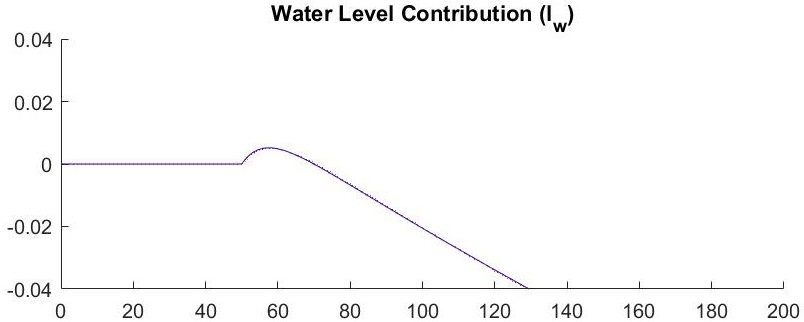
\includegraphics{Modeling/4State/Matlab/Figure22/Figure22-3}}

                Simulation Results using Model from Eq \eqref{eq:Model_1}
                
                \caption{Water Level Contribution to a step change of 10 kg/s in steam flow rate}
                \label{fig:Fig7B}
            \end{center}
        \end{figure}  % Level Water Contribution
        \begin{figure}[ht]
            \begin{center}
                \resizebox{\ScaleABFigThree \textwidth}{!}{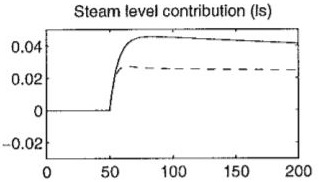
\includegraphics{Modeling/4State/AB_Figures/Figure7/Figure7-AB-5}}
                
                Figure 7 from \r{A}str\"{o}m and Bell's paper, section 5 \cite{Astrom}
                
                \resizebox{\ScaleMLFigThree \textwidth}{!}{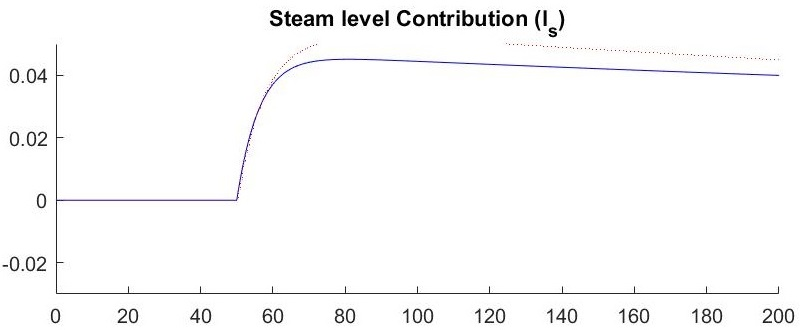
\includegraphics{Modeling/4State/Matlab/Figure22/Figure22-5}}
                
                Simulation Results using Model from Eq \eqref{eq:Model_1}
                
                \caption{Steam Level Contribution to a step change of 10 kg/s in steam flow rate}
                \label{fig:Fig7C}
            \end{center}
        \end{figure}  % Level Steam Contribution    
        
        \begin{figure}[ht]
            \begin{center}
                \resizebox{\ScaleABFigThree \textwidth}{!}{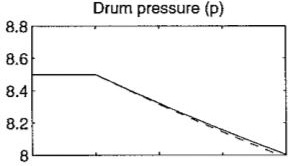
\includegraphics{Modeling/4State/AB_Figures/Figure7/Figure7-AB-2}}
                
                Figure 7 from \r{A}str\"{o}m and Bell's paper, section 5 \cite{Astrom}
                
                \resizebox{\ScaleMLFigThree \textwidth}{!}{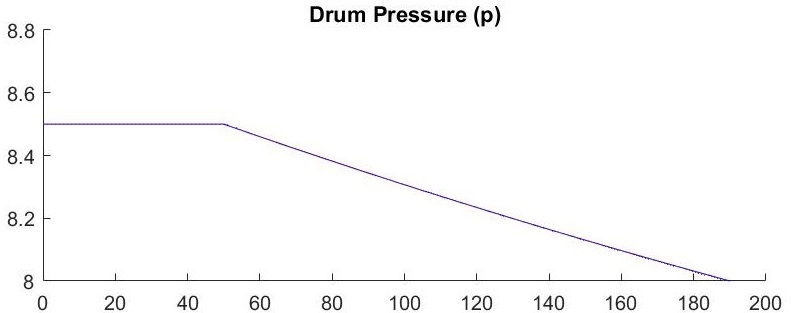
\includegraphics{Modeling/4State/Matlab/Figure22/Figure22-2}}
                
                Simulation Results using Model from Eq \eqref{eq:Model_1}
                
                \caption{Drum Pressure Response to a step change of 10 kg/s in steam flow rate}
                \label{fig:Fig7D}
            \end{center}
        \end{figure}  % Drum Pressure
        \begin{figure}[ht]
            \begin{center}
                \resizebox{\ScaleABFigThree \textwidth}{!}{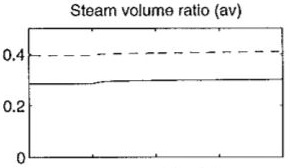
\includegraphics{Modeling/4State/AB_Figures/Figure7/Figure7-AB-4}}
                
                Figure 7 from \r{A}str\"{o}m and Bell's paper, section 5 \cite{Astrom}
                
                \resizebox{\ScaleMLFigThree \textwidth}{!}{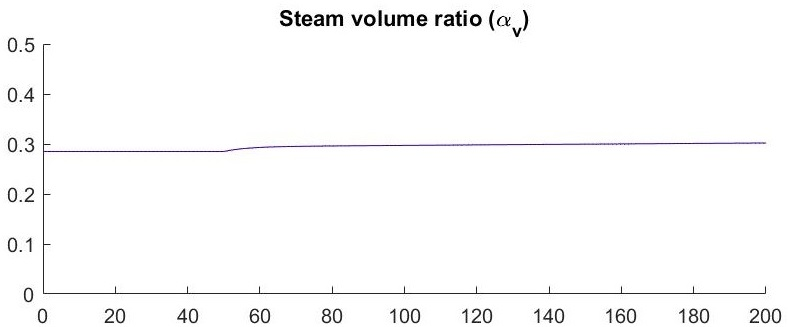
\includegraphics{Modeling/4State/Matlab/Figure22/Figure22-4}}
                
                Simulation Results using Model from Eq \eqref{eq:Model_1}
                
                \caption{Steam Volume Ratio Response to a step change of 10 kg/s in steam flow rate}
                \label{fig:Fig7E}
            \end{center}
        \end{figure}  % Steam Volume Ratio 
        \begin{figure}[ht]
            \begin{center}
                \resizebox{\ScaleABFigThree \textwidth}{!}{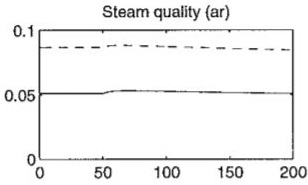
\includegraphics{Modeling/4State/AB_Figures/Figure7/Figure7-AB-6}}
                
                Figure 7 from \r{A}str\"{o}m and Bell's paper, section 5 \cite{Astrom}
                
                \resizebox{\ScaleMLFigThree \textwidth}{!}{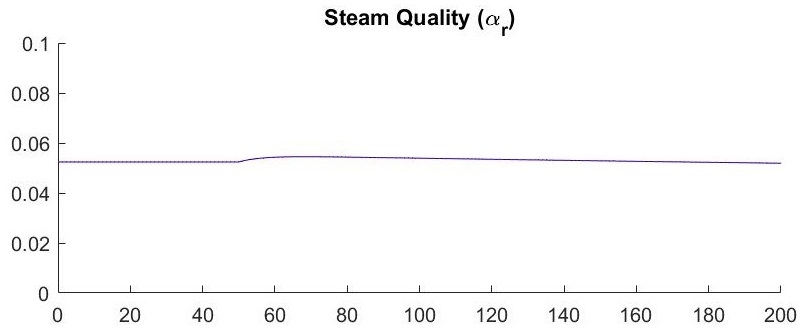
\includegraphics{Modeling/4State/Matlab/Figure22/Figure22-6}}
                
                Simulation Results using Model from Eq \eqref{eq:Model_1}
                
                \caption{Steam Quality Response to a step change of 10 kg/s in steam flow rate}
                \label{fig:Fig7F}
            \end{center}
        \end{figure}  % Steam Quality

        \begin{figure}[ht]
            \begin{center}
                \resizebox{\ScaleABFigThree \textwidth}{!}{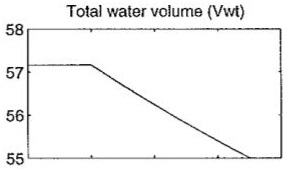
\includegraphics{Modeling/4State/AB_Figures/Figure5/Figure5-AB-2}}
                
                Figure 5 from \r{A}str\"{o}m and Bell's paper, section 5 \cite{Astrom}
                
                \resizebox{\ScaleMLFigThree \textwidth}{!}{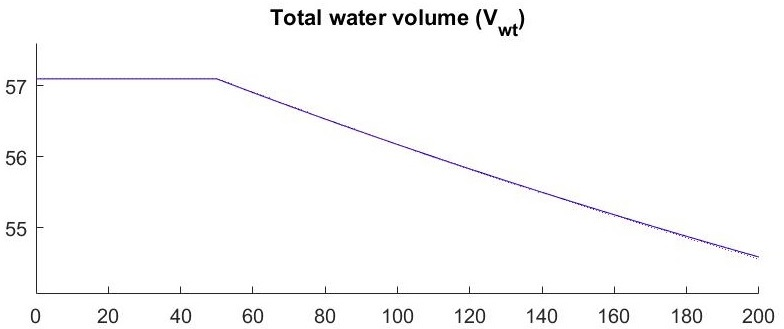
\includegraphics{Modeling/4State/Matlab/Figure21/Figure21-2}}
                
                Simulation Results using Model from Eq \eqref{eq:Model_1}
                
                \caption{Total Water Volume Response to a step change of 10 kg/s in steam flow rate}
                \label{fig:Fig5A}
            \end{center}
        \end{figure}
        \begin{figure}[ht]
            \begin{center}
                \resizebox{\ScaleABFigThree \textwidth}{!}{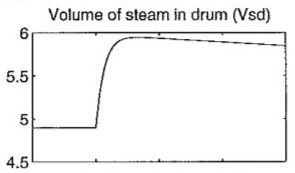
\includegraphics{Modeling/4State/AB_Figures/Figure5/Figure5-AB-4}}
                
                Figure 5 from \r{A}str\"{o}m and Bell's paper, section 5 \cite{Astrom}
                
                \resizebox{\ScaleMLFigThree \textwidth}{!}{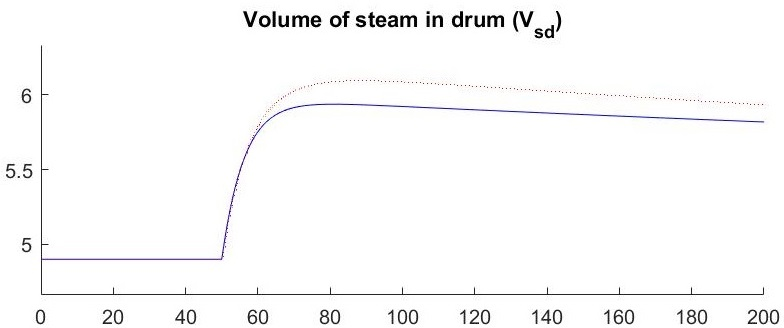
\includegraphics{Modeling/4State/Matlab/Figure21/Figure21-4}}
                
                Simulation Results using Model from Eq \eqref{eq:Model_1}
                
                \caption{Volume of Steam in Drum Response to a step change of 10 kg/s in steam flow rate}
                \label{fig:Fig5B}
            \end{center}
        \end{figure}
        \begin{figure}[ht]
            \begin{center}
                \resizebox{\ScaleABFigThree \textwidth}{!}{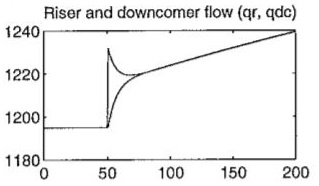
\includegraphics{Modeling/4State/AB_Figures/Figure5/Figure5-AB-5}}
                
                Figure 5 from \r{A}str\"{o}m and Bell's paper, section 5 \cite{Astrom}
                
                \resizebox{\ScaleMLFigThree \textwidth}{!}{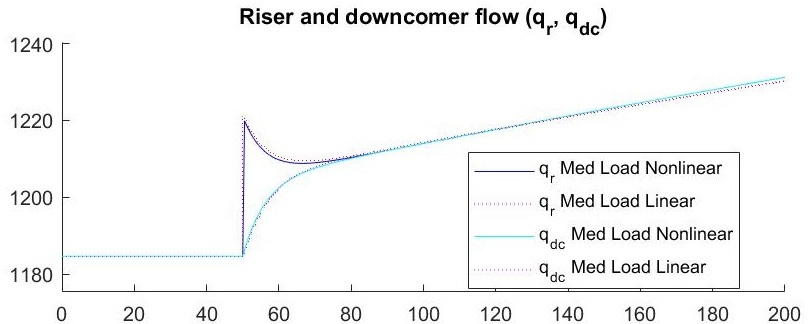
\includegraphics{Modeling/4State/Matlab/Figure21/Figure21-5}}
                
                Simulation Results using Model from Eq \eqref{eq:Model_1}
                
                \caption{Riser and Downcomer Flow Response to a step change of 10 kg/s in steam flow rate}
                \label{fig:Fig5C}
            \end{center}
        \end{figure}
        \begin{figure}[ht]
            \begin{center}
                \resizebox{\ScaleABFigThree \textwidth}{!}{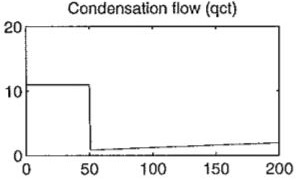
\includegraphics{Modeling/4State/AB_Figures/Figure5/Figure5-AB-6}}
                
                Figure 5 from \r{A}str\"{o}m and Bell's paper, section 5 \cite{Astrom}
                
                \resizebox{\ScaleMLFigThree \textwidth}{!}{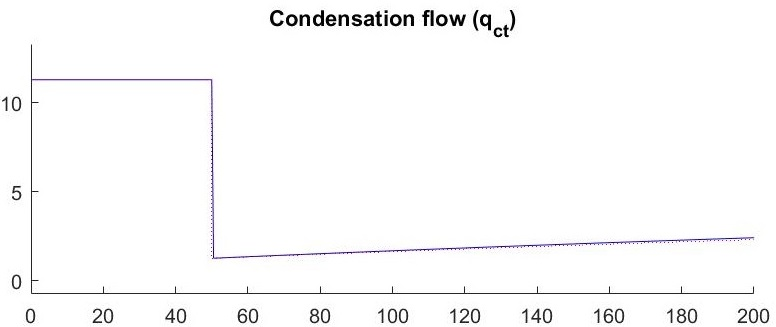
\includegraphics{Modeling/4State/Matlab/Figure21/Figure21-6}}
                
                Simulation Results using Model from Eq \eqref{eq:Model_1}
                
                \caption{Condensation Flow Response to a step change of 10 kg/s in steam flow rate}
                \label{fig:Fig5D}
            \end{center}
        \end{figure}     
            
        10 kg/s in feed water flow Step Responses: Figures \ref{fig:Fig8A}-\ref{fig:Fig8F}
        \begin{figure}[ht]
            \begin{center}
                \resizebox{\ScaleABFigThree \textwidth}{!}{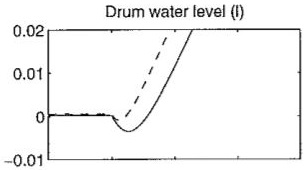
\includegraphics{Modeling/4State/AB_Figures/Figure8/Figure8-AB-1}}
                
                Figure 8 from \r{A}str\"{o}m and Bell's paper, section 5 \cite{Astrom}
                
                \resizebox{\ScaleMLFigThree \textwidth}{!}{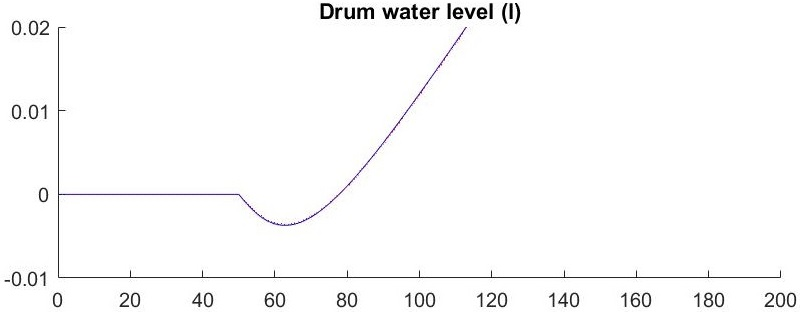
\includegraphics{Modeling/4State/Matlab/Figure32/Figure32-1}}
                
                Simulation Results using Model from Eq \eqref{eq:Model_1}
                
                \caption{Drum Water Level Response to a step corresponding to 10 kg/s in feed water flow rate}
                \label{fig:Fig8A}
            \end{center}
        \end{figure}  % Level
        \begin{figure}[ht]
            \begin{center}
                \resizebox{\ScaleABFigThree \textwidth}{!}{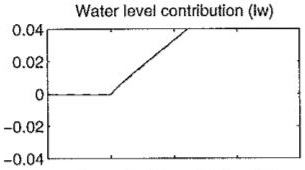
\includegraphics{Modeling/4State/AB_Figures/Figure8/Figure8-AB-3}}
                
                Figure 8 from \r{A}str\"{o}m and Bell's paper, section 5 \cite{Astrom}
                
                \resizebox{\ScaleMLFigThree \textwidth}{!}{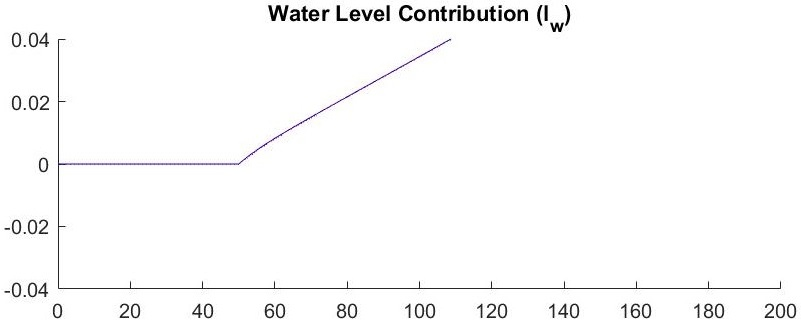
\includegraphics{Modeling/4State/Matlab/Figure32/Figure32-3}}
                
                Simulation Results using Model from Eq \eqref{eq:Model_1}
                
                \caption{Water Level Contribution to a step corresponding to 10 kg/s in feed water flow rate}
                \label{fig:Fig8B}
            \end{center}
        \end{figure}  % Level Water Contribution
        \begin{figure}[ht]
            \begin{center}
                \resizebox{\ScaleABFigThree \textwidth}{!}{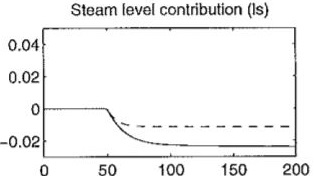
\includegraphics{Modeling/4State/AB_Figures/Figure8/Figure8-AB-5}}
                
                Figure 8 from \r{A}str\"{o}m and Bell's paper, section 5 \cite{Astrom}
                
                \resizebox{\ScaleMLFigThree \textwidth}{!}{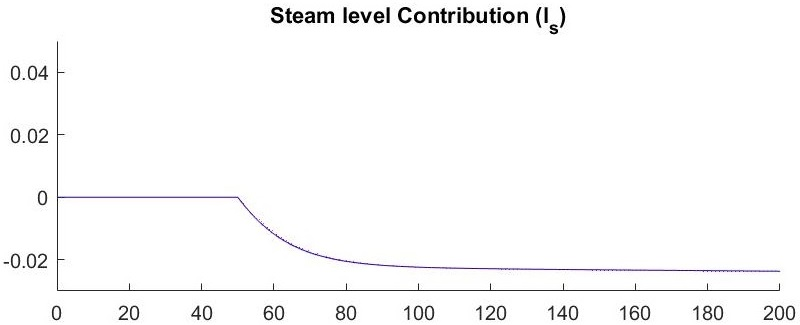
\includegraphics{Modeling/4State/Matlab/Figure32/Figure32-5}}
                
                Simulation Results using Model from Eq \eqref{eq:Model_1}
                
                \caption{Steam Level Contribution to a step corresponding to 10 kg/s in feed water flow rate}
                \label{fig:Fig8C}
            \end{center}
        \end{figure}  % Level Steam Contribution    
        
        \begin{figure}[ht]
            \begin{center}
                \resizebox{\ScaleABFigThree \textwidth}{!}{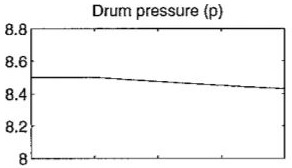
\includegraphics{Modeling/4State/AB_Figures/Figure8/Figure8-AB-2}}
                
                Figure 8 from \r{A}str\"{o}m and Bell's paper, section 5 \cite{Astrom}
                
                \resizebox{\ScaleMLFigThree \textwidth}{!}{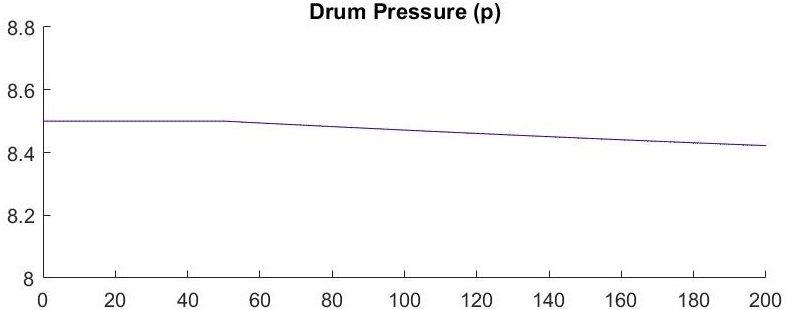
\includegraphics{Modeling/4State/Matlab/Figure32/Figure32-2}}
                
                Simulation Results using Model from Eq \eqref{eq:Model_1}
                
                \caption{Drum Pressure Response to a step corresponding to 10 kg/s in feed water flow rate}
                \label{fig:Fig8D}
            \end{center}
        \end{figure}  % Drum Pressure
        \begin{figure}[ht]
            \begin{center}
                \resizebox{\ScaleABFigThree \textwidth}{!}{\includegraphics{Modeling/4State/AB_Figures/Figure8/Figure8-AB-4}}
                
                Figure 8 from \r{A}str\"{o}m and Bell's paper, section 5 \cite{Astrom}
                
                \resizebox{\ScaleMLFigThree \textwidth}{!}{\includegraphics{Modeling/4State/Matlab/Figure32/Figure32-4}}
                
                Simulation Results using Model from Eq \eqref{eq:Model_1}
                
                \caption{Steam Volume Ratio Response to a step corresponding to 10 kg/s in feed water flow rate}
                \label{fig:Fig8E}
            \end{center}
        \end{figure}  % Steam Volume Ratio 
        \begin{figure}[ht]
            \begin{center}
                \resizebox{\ScaleABFigThree \textwidth}{!}{\includegraphics{Modeling/4State/AB_Figures/Figure8/Figure8-AB-6}}
                
                Figure 8 from \r{A}str\"{o}m and Bell's paper, section 5 \cite{Astrom}
                
                \resizebox{\ScaleMLFigThree \textwidth}{!}{\includegraphics{Modeling/4State/Matlab/Figure32/Figure32-6}}
                
                Simulation Results using Model from Eq \eqref{eq:Model_1}
                
                \caption{Steam Quality Response to a step corresponding to 10 kg/s in feed water flow rate}
                \label{fig:Fig8F}
                
            \end{center}
        \end{figure}  % Steam Quality
        
        10$^O$C Feed Water Step Responses: Figures \ref{fig:Fig9A}-\ref{fig:Fig9F}
        \begin{figure}[ht]
            \begin{center}
                \resizebox{\ScaleABFigThree \textwidth}{!}{\includegraphics{Modeling/4State/AB_Figures/Figure9/Figure9-AB-1}}
                
                Figure 9 from \r{A}str\"{o}m and Bell's paper, section 5 \cite{Astrom}
                
                \resizebox{\ScaleMLFigThree \textwidth}{!}{\includegraphics{Modeling/4State/Matlab/Figure42/Figure42-1}}
                
                Simulation Results using Model from Eq \eqref{eq:Model_1}
                
                \caption{Drum Water Level Response to a step corresponding to 10$^O$C Feed Water Temperature}
                \label{fig:Fig9A}
            \end{center}
        \end{figure}  % Level
        \begin{figure}[ht]
            \begin{center}
                \resizebox{\ScaleABFigThree \textwidth}{!}{\includegraphics{Modeling/4State/AB_Figures/Figure9/Figure9-AB-3}}
                
                Figure 9 from \r{A}str\"{o}m and Bell's paper, section 5 \cite{Astrom}
                
                \resizebox{\ScaleMLFigThree \textwidth}{!}{\includegraphics{Modeling/4State/Matlab/Figure42/Figure42-3}}
                
                Simulation Results using Model from Eq \eqref{eq:Model_1}
                
                \caption{Water Level Contribution to a step corresponding to 10$^O$C Feed Water Temperature}
                \label{fig:Fig9B}
            \end{center}
        \end{figure}  % Level Water Contribution
        \begin{figure}[ht]
            \begin{center}
                \resizebox{\ScaleABFigThree \textwidth}{!}{\includegraphics{Modeling/4State/AB_Figures/Figure9/Figure9-AB-5}}
                
                Figure 9 from \r{A}str\"{o}m and Bell's paper, section 5 \cite{Astrom}
                
                \resizebox{\ScaleMLFigThree \textwidth}{!}{\includegraphics{Modeling/4State/Matlab/Figure42/Figure42-5}}
                
                Simulation Results using Model from Eq \eqref{eq:Model_1}
                
                \caption{Steam Level Contribution to a step corresponding to 10$^O$C Feed Water Temperature}
                \label{fig:Fig9C}
            \end{center}
        \end{figure}  % Level Steam Contribution    
        
        \begin{figure}[ht]
            \begin{center}
                \resizebox{\ScaleABFigThree \textwidth}{!}{\includegraphics{Modeling/4State/AB_Figures/Figure9/Figure9-AB-2}}
                
                Figure 9 from \r{A}str\"{o}m and Bell's paper, section 5 \cite{Astrom}
                
                \resizebox{\ScaleMLFigThree \textwidth}{!}{\includegraphics{Modeling/4State/Matlab/Figure42/Figure42-2}}
                
                Simulation Results using Model from Eq \eqref{eq:Model_1}
                
                \caption{Drum Pressure Response to a step corresponding to 10$^O$C Feed Water Temperature}
                \label{fig:Fig9D}
            \end{center}
        \end{figure}  % Drum Pressure
        \begin{figure}[ht]
            \begin{center}
                \resizebox{\ScaleABFigThree \textwidth}{!}{\includegraphics{Modeling/4State/AB_Figures/Figure9/Figure9-AB-4}}
                
                Figure 9 from \r{A}str\"{o}m and Bell's paper, section 5 \cite{Astrom}
                
                \resizebox{\ScaleMLFigThree \textwidth}{!}{\includegraphics{Modeling/4State/Matlab/Figure42/Figure42-4}}
                
                Simulation Results using Model from Eq \eqref{eq:Model_1}
                
                \caption{Steam Volume Ratio Response to a step corresponding to 10$^O$C Feed Water Temperature}
                \label{fig:Fig9E}
            \end{center}
        \end{figure}  % Steam Volume Ratio 
        \begin{figure}[ht]
            \begin{center}
                \resizebox{\ScaleABFigThree \textwidth}{!}{\includegraphics{Modeling/4State/AB_Figures/Figure9/Figure9-AB-6}}
                
                Figure 9 from \r{A}str\"{o}m and Bell's paper, section 5 \cite{Astrom}
                
                \resizebox{\ScaleMLFigThree \textwidth}{!}{\includegraphics{Modeling/4State/Matlab/Figure42/Figure42-6}}
                
                Simulation Results using Model from Eq \eqref{eq:Model_1}
                
                \caption{Steam Quality Response to a step corresponding to 10$^O$C Feed Water Temperature}
                \label{fig:Fig9F}
            \end{center}
        \end{figure}  % Steam Quality
        
        \clearpage
        
        Using Figures \ref{fig:Fig6A} - \ref{fig:Fig4D} to compare the shape and scale of the graphed outputs from the simulated model and the corresponding output from the \r{A}str\"{o}m and Bell paper, it can be concluded that for a 10 MW fuel flow step increase, the system responses behave similarly. While the specific values may not match exactly due to a difference in calculated Initial Conditions, the same trends are shown on all of the curves. 
        \begin{rem}
            For $u(3) = Q$ the simulated model \eqref{eq:Model_1} has the same step response as the \r{A}str\"{o}m and Bell model
            \label{remark:u3}
        \end{rem}
        
        Using Figures \ref{fig:Fig7A} - \ref{fig:Fig5D} to compare the shape and scale of the graphed outputs from the simulated model and the corresponding output from the \r{A}str\"{o}m and Bell paper, it can be concluded that for a 10 kg/s in steam flow step increase, the system responses behave similarly. While the specific values may not match exactly due to a difference in calculated Initial Conditions, the same trends are shown on all of the curves. 
        \begin{rem}
            For $u(2) = q_s$ the simulated model \eqref{eq:Model_1} has the same step response as the \r{A}str\"{o}m and Bell model
            \label{remark:u2}
        \end{rem}
        
        Using Figures \ref{fig:Fig8A} - \ref{fig:Fig8F} to compare the shape and scale of the graphed outputs from the simulated model and the corresponding output from the \r{A}str\"{o}m and Bell paper, it can be concluded that for a  10 kg/s in feed water flow step increase, the system responses behave similarly. While the specific values may not match exactly due to a difference in calculated Initial Conditions, the same trends are shown on all of the curves. 
        \begin{rem}
            For $u(1) = q_f$ the simulated model \eqref{eq:Model_1} has the same step response as the \r{A}str\"{o}m and Bell model
            \label{remark:u1}
        \end{rem}
        
        Using Figures \ref{fig:Fig9A} - \ref{fig:Fig9F} to compare the shape and scale of the graphed outputs from the simulated model and the corresponding output from the \r{A}str\"{o}m and Bell paper, it can be concluded that for a 10$^O$C Feed Water temperature step  increase, the system responses behave similarly. While the specific values may not match exactly due to a difference in calculated Initial Conditions, the same trends are shown on all of the curves. 
        \begin{rem}
            For $u(4) = t_f$ the simulated model \eqref{eq:Model_1} has the same step response as the \r{A}str\"{o}m and Bell model
            \label{remark:u4}
        \end{rem}
        
        If Remarks \ref{remark:u3} - \ref{remark:u4} are true, and all of the inputs to the model \eqref{eq:Model_1} have been tested then at the specified initial conditions it can be concluded that the model matches the \r{A}str\"{o}m and Bell model.
        
\section{Expanded Model}
    
    The \r{A}str\"{o}m and Bell model uses 4 inputs, $q_f$, $q_s$, $Q$, $t_f$. Expansion upon this allows for a simpler control design. Basic assumptions and methods from previous works allow for the inputs to be lowered down to 2. 
    
    \subsection{Input Simplifications}
    
        \subsubsection{Feedwater}
            Feed-water temperature can usually be considered constant. Once an equilibrium value is found, this can reduce the number of inputs into the model. 
            
            $$ t_{f} = t_{f0} = constant$$
            
            This constant is then used to simplify the inputs from 4 to 3. 
            
        \subsubsection{Steam Flow}
            Steam flow ($q_s$) can be converted from an input to the model if the throttle pressure and throttle valve are modeled. \cite{Iacob}
            
            $$ \aligned
                p - p_t =&K_{sh} \left ( \frac{ q_s}{k_v} \right )^{2} \\
                q_s =& \mu p_t 
            \endaligned$$
            
            $K_v$ becomes a new input from 0-1, which is the throttle valve coefficient. 
            
            Throttle Pressure can be estimated as being between 5\% and 10\% of the drum pressure.\cite{IacobEmail} $K_{sh}$ and $\mu$ can be determined using this information and the above equations. For all simulations, the throttle valve will be left full open, to reduce the number of inputs again. 
            
            $$ \aligned
                K_{sh} =& 0.0013  \\
                \mu    =& 6.77 \\ 
                k_v    =& 1
            \endaligned$$
                

            This then produces: 
            
            $$p  = K_{sh} q_s^{2} + \frac{ q_s}{\mu} \Longrightarrow  q_s = f(p)$$
            %$$\frac { \sqrt{ K_{sh} p \mu^2 4+1} - 1 } {2 K_{sh} \mu}$$
            
            This function further simplifies the inputs from 3 (see Feedwater above) to 2, as $q_s$ is now a direct function of $p$. 
            
        \subsubsection{Valve Dynamics}
            The remaining inputs are controlled by valves, so first order approximations for the valve movement was added. In the below, $T_{v_{Q }}$ and $T_{v_{fw}}$ are the valve time constants.  
            
            $$ \dot{Q}_{valve}  = \frac{\left(  Q_{valve}  - Q       \right)}{T_{v_{Q }}}$$
            $$ \dot{FW}_{valve} = \frac{\left( FW_{valve}  - q_{fw}  \right)}{T_{v_{fw}}}$$
            
            This can be put into matrix form to in the following way:
            \begin{equation}
                \frac{\mathrm{d} }{\mathrm{d} t} 
                \left [ \begin{matrix} Q_{valve} \\ FW_{valve} \end{matrix} \right ]  
                =
                \left[ \begin{matrix} \frac{\left(  Q_{valve}  - Q       \right)}{T_{v_{Q }}} \\\frac{\left( FW_{valve}  - q_{fw}  \right)}{T_{v_{fw}}}   \end{matrix} \right]
                \label{eq:Valve_model_A}
            \end{equation}
            These were then incorporated into the state equation, creating a 6 function nonlinear differential equation, with 6 states and 2 inputs. 
            
            $$ \begin{matrix} V_{wt} & p& \alpha_r& V_{sd} & Q & q_{fw}\end{matrix} $$
            $$ \begin{matrix} Q_{valve} & FW_{valve} \end{matrix} $$
        
    \subsection{Expanded Model with Simplified Inputs}
        Combining Equations \ref{eq:Model_1} and \ref{eq:Valve_model_A} results in the following:
        \begin{equation}
            \label{eq:Valve_Model_1}
            \frac{\mathrm{d} }{\mathrm{d} t} 
            \left [ \begin{matrix} \left [ \begin{matrix} V_{wt}\\ p\\ \alpha_r\\ V_{sd}\end{matrix} \right ]  \\ \left [ \begin{matrix} Q_{valve} \\ FW_{valve} \end{matrix} \right ] \end{matrix} \right ]  
            =
            \left [ \begin{matrix}  \left [ \begin{matrix}e_{11}& e_{12}& 0& 0 \\ e_{21}& e_{22}& 0& 0 \\ 0 & e_{32}& e_{33}& 0 \\ 0 & e_{42}& e_{43}& e_{44}\end{matrix} \right ] ^{-1} \left [ \begin{matrix} q_f  - q_s \\ Q + q_f h_f  - q_s h_s\\ Q + \alpha_r h_c q_{dc} \\ \frac{\rho_s}{T_d}  \left ( V_{sd}^0  - V_{sd}\right ) + \frac{h_f - h_w}{h_c}q_f \end{matrix} 
            \right ] \\  \left[ \begin{matrix} \frac{\left(  Q_{valve}  - Q       \right)}{T_{v_{Q }}} \\\frac{\left( FW_{valve}  - q_{fw}  \right)}{T_{v_{fw}}}   \end{matrix} \right]  \end{matrix} \right ]
        \end{equation}
     
        It should be noted that Equation \ref{eq:Valve_Model_1} is in terms of
        $$ \dot{x} = f\left (x, u\right)$$
        Where:
        $$ x = \left [\begin{matrix} V_{wt} & p & \alpha_r & V_{sd} & Q & q_{fw}\end{matrix} \right]^T$$
        $$ u = \left [\begin{matrix} Q_{valve} & FW_{valve} \end{matrix} \right]^T$$        
        
        This is the form of a Nonlinear-Time-Invariant State Space system. 
        
        A list of simplifications made for the final model used \eqref{eq:Valve_Model_1} are as follows:
    
        \begin{itemize}
          \item Feed water Valve is treated as a first order system compared to Feed water Flow
          \item Fuel Valve is treated as a first order system compared to Heat transfer into the boiler. This is an oversimplification of the fuel flow dynamics, which consist of fuel flow and air flow. Air flow is normally controlled by excess flue oxygen and the stoichiometric ratio to fuel flow.  
          \item Feed water Temperature is treated as constant
          \item Steam Flow is estimated based off of throttle pressure
          \item Properties of water are modeled based off of numerical evidence
        \end{itemize}        
    
    \subsection{Open Loop Step Responses to Expanded Model}
    
        The model used in Eq. \ref{eq:Valve_Model_1} was simulated with step inputs, the results are the following figures. 
        
        Figures \ref{fig:Valve_Open1A} - \ref{fig:Valve_Open1E} use the model \eqref{eq:Valve_Model_1}, while Figures \ref{fig:Fig6A} - \ref{fig:Fig6F} uses the model \eqref{eq:Model_1}. Both sets of figures use the same step input of $Q$ = 10 MW, however the expanded model uses a first order dynamic delay. 
        
        Figures \ref{fig:Valve_Open2A} - \ref{fig:Valve_Open2E} use the model \eqref{eq:Valve_Model_1}, while Figures \ref{fig:Fig8A} - \ref{fig:Fig8F} uses the model \eqref{eq:Model_1}. Both sets of figures use the same step input of $q_f$ = 10 kg/s, however the expanded model uses a first order dynamic delay. 
        
        \begin{figure}[ht]
            \begin{center}
                \resizebox{\ScaleMLFigThree \textwidth}{!}{\includegraphics{Modeling/6State/Matlab/Figure81/Figure81-1}}
                
                Short Term Step Response
                
                \resizebox{\ScaleMLFigThree \textwidth}{!}{\includegraphics{Modeling/6State/Matlab/Figure82/Figure82-1}}
                
                Long Term Step Response
                
                \caption{Drum Water Level Response to a step corresponding to 10 MW in fuel flow rate}
                \label{fig:Valve_Open1A}
            \end{center}
            Figure \ref{fig:Valve_Open1A} should be directly compared to Figure \ref{fig:Fig6A}. This shows the shrink/swell effect, in how level initially reacts in one direction, however it ultimately trends towards the opposite direction.
        \end{figure}  % A Level
        
        
        \begin{figure}[ht]
            \begin{center}
                \resizebox{\ScaleMLFigThree \textwidth}{!}{\includegraphics{Modeling/6State/Matlab/Figure81/Figure81-2}}
                
                Short Term Step Response
                
                \resizebox{\ScaleMLFigThree \textwidth}{!}{\includegraphics{Modeling/6State/Matlab/Figure82/Figure82-2}}
                
                Long Term Step Response
                
                \caption{Drum Pressure Response to a step corresponding to 10 MW in fuel flow rate}
                \label{fig:Valve_Open1B}
            \end{center}
            Figure \ref{fig:Valve_Open1B} should be directly compared to Figure \ref{fig:Fig6D}, the initial response matches what was seen in the \r{A}str\"{o}m and Bell paper and pressure eventually reaches a stable settling point.
        \end{figure}  % B Pressure  
        
        \begin{figure}[ht]
            \begin{center}
                \resizebox{\ScaleMLFigThree \textwidth}{!}{\includegraphics{Modeling/6State/Matlab/Figure81/Figure81-3}}
                
                Short Term Step Response
                
                \resizebox{\ScaleMLFigThree \textwidth}{!}{\includegraphics{Modeling/6State/Matlab/Figure82/Figure82-3}}
                
                Long Term Step Response
                
                \caption{Volume of Total Water Response to a step corresponding to 10 MW in fuel flow rate}
                \label{fig:Valve_Open1C}
            \end{center}
            Figure \ref{fig:Valve_Open1C} is not directly comparable to a figure from the \r{A}str\"{o}m and Bell paper, however it makes sense that if the feed water valve is held constant but more heat is added that water will eventually leave the system in the form of steam. 
        \end{figure}  % C Volume of Water Total
        
        \begin{figure}[ht]
            \begin{center}
                \resizebox{\ScaleMLFigThree \textwidth}{!}{\includegraphics{Modeling/6State/Matlab/Figure81/Figure81-4}}
                
                Short Term Step Response
                
                \resizebox{\ScaleMLFigThree \textwidth}{!}{\includegraphics{Modeling/6State/Matlab/Figure82/Figure82-4}}
                
                Long Term Step Response
                
                \caption{Steam Quality Response to a step corresponding to 10 MW in fuel flow rate}
                \label{fig:Valve_Open1D}
            \end{center}
            Figure \ref{fig:Valve_Open1D} should be directly compared to Figure \ref{fig:Fig6F}, the initial response matches what was seen in the \r{A}str\"{o}m and Bell paper and steam quality eventually reaches a stable settling point.
        \end{figure}  % D Steam Quality 
        
        \begin{figure}[ht]
            \begin{center}
                \resizebox{\ScaleMLFigThree \textwidth}{!}{\includegraphics{Modeling/6State/Matlab/Figure81/Figure81-5}}
                
                Short Term Step Response
                
                \resizebox{\ScaleMLFigThree \textwidth}{!}{\includegraphics{Modeling/6State/Matlab/Figure82/Figure82-5}}
                
                Long Term Step Response
                
                \caption{Volume of Steam in the Drum Response to a step corresponding to 10 MW in fuel flow rate}
                \label{fig:Valve_Open1E}
            \end{center}
            Figure \ref{fig:Valve_Open1E} should be directly compared to Figure \ref{fig:Fig6C}, as the volume of steam in the drum is directly proportional to the steam level contribution. As seen in the level plots (Figure \ref{fig:Valve_Open1A}) the shirnk/swell effect can be partially seen here. 
        \end{figure}  % E Volume of Steam Drum     
        
        \begin{figure}[ht]
            \begin{center}
                \resizebox{\ScaleMLFigThree \textwidth}{!}{\includegraphics{Modeling/6State/Matlab/Figure91/Figure91-1}}
                
                Short Term Step Response
                
                \resizebox{\ScaleMLFigThree \textwidth}{!}{\includegraphics{Modeling/6State/Matlab/Figure92/Figure92-1}}
                
                Long Term Step Response
                
                \caption{Drum Water Level Response to a step corresponding to 10 kg/s feed water flow rate}
                \label{fig:Valve_Open2A}
            \end{center}
            Figure \ref{fig:Valve_Open2A} should be directly compared to Figure \ref{fig:Fig8A}. This shows the shrink/swell effect, in how level initially reacts in one direction, however it ultimately trends towards the opposite direction.
        \end{figure}  % A Level
        
        \begin{figure}[ht]
            \begin{center}
                \resizebox{\ScaleMLFigThree \textwidth}{!}{\includegraphics{Modeling/6State/Matlab/Figure91/Figure91-2}}
                
                Short Term Step Response
                
                \resizebox{\ScaleMLFigThree \textwidth}{!}{\includegraphics{Modeling/6State/Matlab/Figure92/Figure92-2}}
                
                Long Term Step Response
                
                \caption{Drum Pressure Response to a step corresponding to 10 kg/s feed water flow rate}
                \label{fig:Valve_Open2B}
            \end{center}
            Figure \ref{fig:Valve_Open2B} should be directly compared to Figure \ref{fig:Fig8D}, the initial response matches what was seen in the \r{A}str\"{o}m and Bell paper and pressure eventually reaches a stable settling point.
        \end{figure}  % B Pressure 
        
        \begin{figure}[ht]
            \begin{center}
                \resizebox{\ScaleMLFigThree \textwidth}{!}{\includegraphics{Modeling/6State/Matlab/Figure91/Figure91-3}}
                
                Short Term Step Response
                
                \resizebox{\ScaleMLFigThree \textwidth}{!}{\includegraphics{Modeling/6State/Matlab/Figure92/Figure92-3}}
                
                Long Term Step Response
                
                \caption{Volume of Total Water Response to a step corresponding to 10 kg/s feed water flow rate}
                \label{fig:Valve_Open2C}
            \end{center}
            Figure \ref{fig:Valve_Open2C} is not directly comparable to a figure from the \r{A}str\"{o}m and Bell paper, however it makes sense that if the feed water increased from a stable operating point and all other inputs are held constant, then more water will eventually fill the drum. 
        \end{figure}  % C Volume of Water Total
        
        \begin{figure}[ht]
            \begin{center}
                \resizebox{\ScaleMLFigThree \textwidth}{!}{\includegraphics{Modeling/6State/Matlab/Figure91/Figure91-4}}
                
                Short Term Step Response
                
                \resizebox{\ScaleMLFigThree \textwidth}{!}{\includegraphics{Modeling/6State/Matlab/Figure92/Figure92-4}}
                
                Long Term Step Response
                
                \caption{Steam Quality Response to a step corresponding to 10 kg/s feed water flow rate}
                \label{fig:Valve_Open2D}
            \end{center}
            Figure \ref{fig:Valve_Open2D} should be directly compared to Figure \ref{fig:Fig8F}, the initial response matches what was seen in the \r{A}str\"{o}m and Bell paper and steam quality eventually reaches a stable settling point.
        \end{figure}  % D Steam Quality 
        
        \begin{figure}[ht]
            \begin{center}
                \resizebox{\ScaleMLFigThree \textwidth}{!}{\includegraphics{Modeling/6State/Matlab/Figure91/Figure91-5}}
               
                Short Term Step Response
                
                \resizebox{\ScaleMLFigThree \textwidth}{!}{\includegraphics{Modeling/6State/Matlab/Figure92/Figure92-5}}
                
                Long Term Step Response
                
                \caption{Volume of Steam in the Drum Response to a step corresponding to 10 kg/s feed water flow rate}
                \label{fig:Valve_Open2E}
            \end{center}
            Figure \ref{fig:Valve_Open2E} should be directly compared to Figure \ref{fig:Fig8C}, as the volume of steam in the drum is directly proportional to the steam level contribution. 
        \end{figure}  % E Volume of Steam Drum  
        
        

        \clearpage
        %What can be seen in Figure \ref{fig:Valve_Open1B} and \ref{fig:Valve_Open2B} are the long term responses of step inputs of Megawatts (in terms of heat input) and feed water flow. Figure \ref{fig:Valve_Open1B} shows expected values eventually becoming stable, such as drum pressure. What is worth noting though is the early dynamics, which can be see in in Figure \ref{fig:Valve_Open1A} and in particular the drum water level behaves in direct opposition to how it behaves in the long term. Initially the drum water rises, sees some effects of shrink/swell, but overall rises. The long term response though shows drum level as near constantly decreasing. Figure\ref{fig:Valve_Open2B} shows expected values eventually becoming stable, and drum level constantly rising, which is to be expected if water is constantly added into the drum. The early responses are also acting differently to the overall trend, but to a lesser extent.
        
        These simulations do not take into account that the drum has a completely finite volume to fill nor does it take into account the possibility of bursting from high pressure. Future work could expand upon this, however this is not necessary for this paper. The goal of these long term simulations was to determine that the shrink/swell effect was occurring and on what timescale would it be necessary to see those effects. Future simulations will be well within physical controllable ranges. 
